\subsection{Higher dimensional dynamic systems}
\subsubsection{Linear Systems}
1D flows are qualitatively simple - either the system moves in one direction or it stops. This is different in higher dimensions, where one may observe a more complex behaviour.\\
We first discuss the most simple system in 2D; i.e. a linear system
\begin{align*}
	\dot{x}&=ax+by\\
	\dot{y}&=cx+dy
\end{align*}
This system can be rewritten as:
\begin{equation*}
	\dot{\vec{x}}=\mat{A}\vec{x}\qquad\text{where}\quad\mat{A}=\begin{pmatrix} a & b \\ c & d \end{pmatrix}\quad\text{and}\quad\vec{x}=\begin{pmatrix}x\\ y\end{pmatrix}
\end{equation*}
Linearity implies that $\vec{x}=c\vec{x}_1+c\vec{x_2}$ is a solution of the system if $\vec{x}_1$ and $\vec{x}_2$ are solutions of the system ($c_1,c_2$ are arbitrary parameters)\vspace{0.5 cm}\\
\textbf{\underline{\smash{Example}}}: Oscillator
\begin{equation*}
	m\ddot{x}+kx=0\begin{cases}\dot{x}=v\\\dot{v}=-\frac{k}{m}x\end{cases}
\end{equation*}
Again, we obtain a vectorfield which we want to analyse in the following:\\
At the $x$-axis (i.e. $v=0$) we get:
\begin{equation*}
	\dot{x}=0\qquad \dot{v}=-\omega^2 x\qquad\qquad \left(\omega^2=\frac{k}{m}\right)
\end{equation*}
Similarly, we get:
\begin{align*}
	\dot{x}&=v \quad\text{at the $v$-axis}\\
	\dot{v}&=0
\end{align*}
Usign similar arguments we get:
\begin{figure}[H]
	\centering
	\begin{multicols}{2}
		\begin{figure}[H]
			\centering
			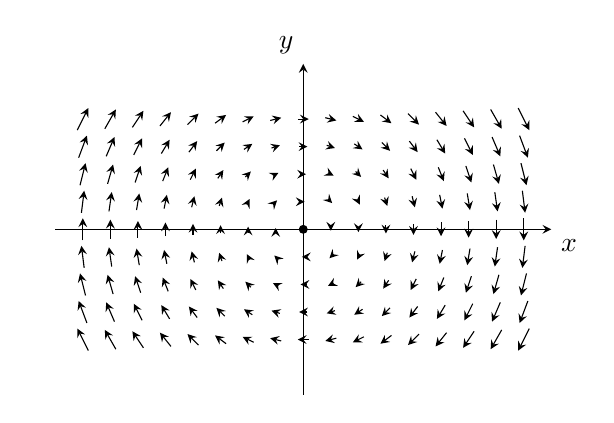
\begin{tikzpicture}[scale=0.7,>=stealth]
				\draw[->] (-4.5,0)--(4.5,0)node[below right]{$x$};
				\draw[->] (0,-3)--(0,3)node[above left]{$y$};
				\draw[fill=black] (0,0)circle(2pt);
				\begin{scope}
					\path[clip,domain=0:360] (-0.2,-0.2)--(0.2,-0.2)--(0.2,0.2)--(-0.2,0.2)(-5,-3)--(-5,3)--(5,3)--(5,-3)--(-5,-3)(-0.2,-0.2);
					\foreach \x in {-4,-3.5,...,4}{
						\foreach \y in {-2,-1.5,...,2}{
							\draw[->](\x-0.05*\y,\y+0.05*\x)--(\x+0.05*\y,\y-0.05*\x);
						}
					}
				\end{scope}
			\end{tikzpicture}
		\end{figure}\columnbreak
		\begin{figure}[H]
			\centering
			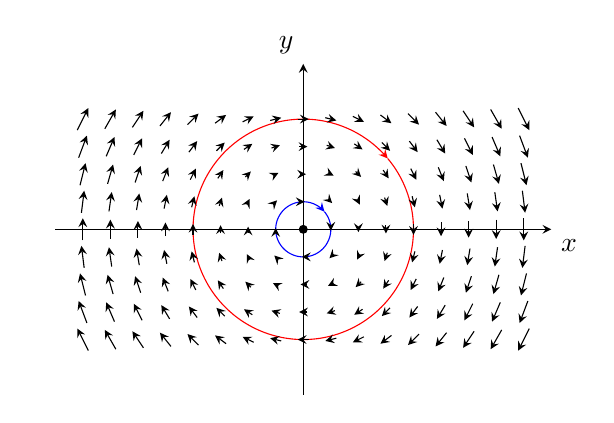
\begin{tikzpicture}[scale=0.7,>=stealth, ]
				\draw[->] (-4.5,0)--(4.5,0)node[below right]{$x$};
				\draw[->] (0,-3)--(0,3)node[above left]{$y$};
				\draw[fill=black] (0,0)circle(2pt);
				\draw[red,->,domain=400:40,samples=200] plot({2*cos(\x)},{2*sin(\x)});
				\draw[blue,->,domain=400:40,samples=200] plot({0.5*cos(\x)},{0.5*sin(\x)});
				\begin{scope}
					\path[clip,domain=0:360] (-0.2,-0.2)--(0.2,-0.2)--(0.2,0.2)--(-0.2,0.2)(-5,-3)--(-5,3)--(5,3)--(5,-3)--(-5,-3)(-0.2,-0.2);
					\foreach \x in {-4,-3.5,...,4}{
						\foreach \y in {-2,-1.5,...,2}{
							\draw[->](\x-0.05*\y,\y+0.05*\x)--(\x+0.05*\y,\y-0.05*\x);
						}
					}
				\end{scope}
			\end{tikzpicture}
		\end{figure}
	\end{multicols}
\end{figure}
\noindent\textbf{\underline{\smash{Classification of linear systems}}}:\vspace{0.2 cm}\\
We are now going to classify all possible phase portraits in 2D-linear systems\\
Straight line trajectories:
\begin{equation*}
	\vec{x}(t)=e^{\lambda t}\vec{v}
\end{equation*}
$\vec{v}$ constant vector, $\lambda$: growth rate\vspace{0.2cm}\\
We take this form as an ansatz for our linear equation:
\begin{equation*}
	\vec{x}(t)=\lambda e^{\lambda t}\vec{v}=\mat{A}\vec{x}(t)=\mat{A}e^{\lambda t}\vec{v}
\end{equation*}
\begin{equation*}
	\leadsto \lambda\vec{v}=\mat{A}\vec{v}
\end{equation*}
This eigenvalue problem can be easily solved. The eigenvalues are given by:
\begin{equation*}
	\lambda_{1,2}=\frac{\tau\pm\sqrt{\tau^2-4\Delta}}{2}\qquad (\tau=\text{tr}(A)=a+d,\Delta=\text{det}(A)=ad-bc)
\end{equation*}
The general solution of the system is given by
\begin{equation*}
	\vec{x}(t)=c_1e^{\lambda_1t}\vec{v}_1+c_2e^{\lambda_2t}\vec{v}_2
\end{equation*}
where $\vec{v}_1,\vec{v}_2$ are the eigenvectors of the system.\\
The eigenvalues determine obviously the properties of the sytem.\\
We obtain the following classification of fixed points:
\begin{figure}[H]
	\centering
	\begin{tikzpicture}
		\draw[->](-5,0)--(5,0)node[below right]{$\Delta$};
		\draw[->](0,-3)--(0,3)node[above left]{$\tau$};
		\node[left] at (-0.2,1){saddle points};
		\draw[domain={-sqrt(5)}:{sqrt(5)},samples=100] plot({(\x)^2},\x);
		\node[right] at (2,3){unstable nodes};
		\node[right] at (2,1){stable nodes};
		\node[right] at (2,-1){stable spirals};
		\node[right] at (2,-3){unstable spirals};
		\node[above right] at (2,0){centers};
	\end{tikzpicture}
\end{figure}
The classification can be obtained by using the following equations
\begin{equation*}
	\lambda_{1,2}=\frac{1}{2}\left(\tau\pm\sqrt{\tau^2-4\Delta}\right),\quad \Delta=\lambda_1\lambda_2,\tau=\lambda_1+\lambda_2
\end{equation*}
$\Delta<0$: The eigenvalues are real and have opposite sign $\to$ saddle point
\begin{figure}[H]
	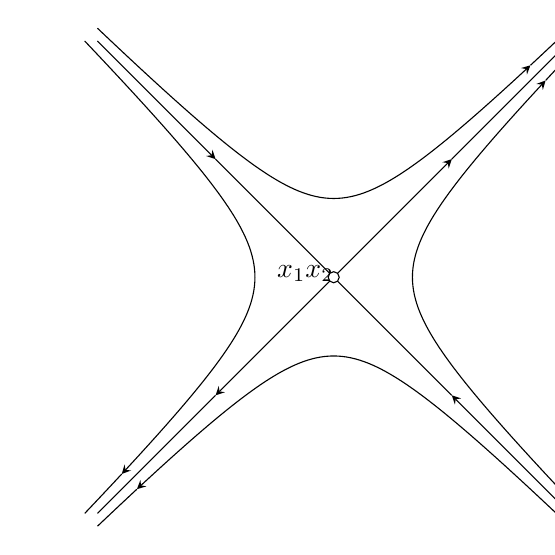
\begin{tikzpicture}[>=stealth]
		\koord{-4}{4}{-3}{3}{$x_1$}{$x_2$};
		\draw[->] (-3,3)--(-1.5,1.5);
		\draw (-1.5,1.5)--(0,0);
		\draw[->] (3,-3)--(1.5,-1.5);
		\draw (1.5,-1.5)--(0,0);
		\draw[->] (0,0)--(-1.5,-1.5);
		\draw (-1.5,-1.5)--(-3,-3);
		\draw[->] (0,0)--(1.5,1.5);
		\draw (1.5,1.5)--(3,3);
		\draw[fill=white] (0,0)circle(2pt);x	
		\draw[->,domain=-3:2.5,samples=100] plot(\x,{sqrt(1+(\x)^2)});
		\draw[domain=2.5:3,samples=20] plot(\x,{sqrt(1+(\x)^2)});
		\draw[->,domain=3:-2.5,samples=100] plot(\x,{-sqrt(1+(\x)^2)});
		\draw[domain=-2.5:-3,samples=20] plot(\x,{-sqrt(1+(\x)^2)});
		\draw[->,domain=3:-2.5,samples=100] plot({-sqrt(1+(\x)^2)},\x);
		\draw[domain=-2.5:-3,samples=20] plot({-sqrt(1+(\x)^2)},\x);
		\draw[->,domain=-3:2.5,samples=100] plot({sqrt(1+(\x)^2)},\x);
		\draw[domain=2.5:3,samples=20] plot({sqrt(1+(\x)^2)},\x);
	\end{tikzpicture}
\end{figure}
\noindent If $\Delta>0$ the eigenvalues are either real with the same \\
sign (nodes) ($\tau^2-4\Delta>0$) or complex conjugate (spirals and centers, $\tau^2-4\Delta<0$)\\
$\tau<0:$ Both eigenvalues have negative real parts $\to$ stable spirals\\
$\tau>0:$ unstable nodes and spirals\\
$\tau=0:$ stable\\
$\Delta=0$: At least one of the eigenvalues is zero $\to$ origin is not an isolated fixed point\\
\underline{Phase plane}: From now on we consider non-linear two-dimensional systems\\
\underline{Phase-Portrait}: Vectorfield:
\begin{align*}
	\vec{x_1}&=f_1(x_1,x_2)\\
	\vec{x_2}&=f_2(x_1,x_2)
\end{align*}
\begin{equation*}
	\text{or }\quad \dot{\vec{x}}=\vec{f}(\vec{x})
\end{equation*}
where $\vec{x}=(x_1,x_2)$ and $\vec{f}(\vec{x})=(f_1(\vec{x}),f_2(\vec{x}))$\\
A solution $\vec{x}(t)$ of $(\ast)$ corresponds to a trajectory in the 2D phaseplane\\
Typically $(\ast)$ cannot be solved for non-linear systems. One way to approach the equation $(\ast)$ is numerical, e.g. the Runge-Kutta method
\begin{equation*}
	\vec{x}_{n+1}=\vec{x}_n+\frac{1}{6}\left(\vec{k}_1+2\vec{k}_2+2\vec{k}_3+\vec{k}_4\right)+\mathcal{O}\left((\Delta t)^5\right)
\end{equation*}
where
\begin{align*}
	\vec{k}_1&=\vec{f}\left(\vec{x}_n\right)\Delta t & \vec{k}_2&=\vec{f}\left(\vec{x}_n+\frac{1}{2}\vec{k}_1\right)\Delta t\\
	\vec{k}_3&=\vec{f}\left(\vec{x}_n+\frac{1}{2}\vec{k}_2\right)\Delta t & \vec{k}_4&=\vec{f}\left(\vec{x}_n+\vec{k}_3\right)\Delta t
\end{align*}
\underline{Example}: We consider the system
\begin{equation*}
	\dot{x}=x+e^{-y} \qquad \dot{y}=-y
\end{equation*}
Fixed point: $\dot{x}=0,\dot{y}=0\quad\Rightarrow\quad y=0; x=-1$ corresponds to a fixed point\\
The solution of $\dot{y}=-y$ is given by $y(t)=y_0e^{-t}$\\
$\underset{t\to\infty}{\leadsto} y(t)=0\underset{t>>1}{\leadsto}\dot{x}=x+1$ This equation has exponentially growing solution, which indicates, that the fixed point is unstable.\\
The phaseportrait can be construted by using the following consideration:
\begin{enumerate}[label={$\arabic*)$}]
	\item We consider $y_0=0\leadsto \dot{y}=0$ for all times
	\item To sketch the phase space it is useful to plot the mill lines, i.e. the curves where either $\dot{x}=0$ or $\dot{y}=0$.
		\begin{align*}
			\dot{y}=0 &\leadsto \text{ horizontal flow}\\
			\dot{x}=0 &\leadsto \text{ vertical flow.}\\
			\text{We have } x+e^{-y}=0&\leadsto y=\ln\left(-\frac{1}{x}\right)
		\end{align*}
\end{enumerate}
\begin{center}
	\begin{figure}[H]
		\centering
		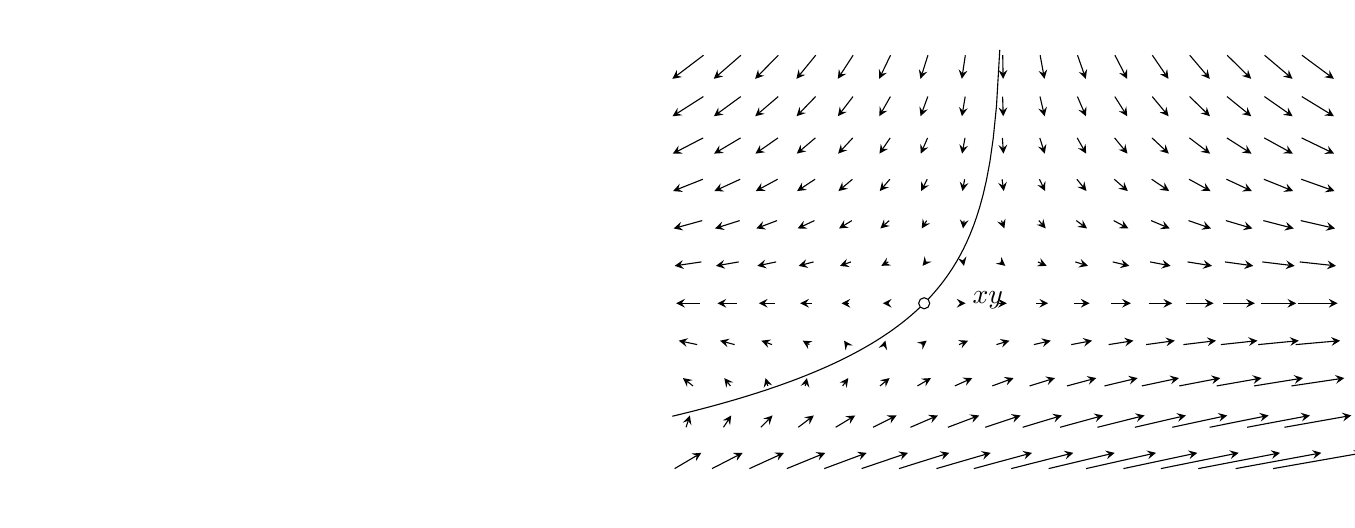
\begin{tikzpicture}[>=stealth]
			\koord{-4.5}{4.5}{-2.5}{3.5}{$x$}{$y$};
			\draw[domain={-0.04}:-4.2,samples=100] plot(\x,{ln(-1/\x)});
			\draw[fill=white] (-1,0)circle(2pt);
			\begin{scope}
				%\clip (-1.2,-0.2)--(-1.2,0.2)--(-0.8,0.2)--(-0.8,-0.2)--(-1.2,-0.2)(-6,-5)--(-6,5)--(6,5)--(6,-5)--(-6,-5)(-1.2,-0.2);
				%\path[clip,domain=0:360,xshift=-1cm] (-0.2,-0.2)--(0.2,-0.2)--(0.2,0.2)--(-0.2,0.2)(-5,-4)--(-5,4)--(7,4)--(7,-4)--(-5,-4)(-0.2,-0.2);
				\path[clip] (-1.2,-0.2)--(-0.8,-0.2)--(-0.8,0.2)--(-1.2,0.2)--(-1.2,-0.2)(-4.5,-2.5)--(-4.5,3.5)--(4.5,3.5)--(4.5,-2.5)--(-4.5,-2.5)(-12,-0.2);
				%\draw (-1.2,-0.2)--(-1.2,0.2)--(-0.8,0.2)--(-0.8,-0.2)--(-1.2,-0.2)--(-6,-5)--(-6,5)--(6,5)--(6,-5)--(-6,-5)--(-1.2,-0.2);
				\foreach \x in {-4,-3.5,...,4}{
					\foreach \y in {-2,-1.5,...,3}{
						\draw[->] ({\x-0.05*(\x+exp(-\y))},{\y+0.05*\y})--({\x+0.05*(\x+exp(-\y))},{\y-0.05*\y});
					}
				}
			\end{scope}
		\end{tikzpicture}
	\end{figure}
\end{center}
\large{\textbf{\underline{\smash{Existence, uniqueness and topological consequences}}}}\normalsize{}\vspace{0.2cm}\\
\textbf{\underline{\smash{Theorem}}}: Consider the initial value problem $\dot{\vec{x}}=\vec{f}(\vec{x}); \vec{x}(0)=\vec{x}_0$\\
Suppose that $\vec{f}$ is continuous and that all its partial derivatives $\frac{\partial f_i}{\partial x_j},\ i,j=1,2,\ldots,n$ are continuous for $\vec{x}$ in some open connected set $D\in\R^n$. Then for $\vec{x}_0\in D$, the initial value problem has a solution $x(t)$ on some time interval $]-\tau,\tau[$ about $t=0$, and the solution is unique.\\
\underline{\smash{Remark}}:
\begin{enumerate}[label={$\arabic*)$}]
	\item The theorem implies that the trajectories don't intersect.
	\item The Poincaré-Bendixson theorem states, that if a trajectory is confined to a closed bounded region, then the trajectory must eventually approach a closed orbit.
\end{enumerate}
\textbf{\underline{\smash{Fixed points and linearization}}}\vspace{0.2cm}\\
\underline{\smash{Linearization}}: Approximation of the phase portrait near a fixed point by a corresponding linear system.\\
Consider:
\begin{align*}
	\dot{x}&=f(x,y) & f(x^\ast,y^\ast)=&0=g(x^\ast,y^\ast)\\
	\dot{y}&=g(x,y) & u=x-x^\ast&;v=y-y^\ast
\end{align*}
$\dot{u}=\dot{x}=f(x^\ast+u,y^\ast+v)=f(x^\ast,y^\ast)+u\partial_x f+v\partial_yf+\mathcal{O}\left(u^2,v^2,uv\right)$ analogous for $\dot{v}$.\\
Therefore the linearized system is given by
\begin{equation*}
	\begin{pmatrix} \dot{u} \\\dot{v}\end{pmatrix}=A\begin{pmatrix}u\\ v\end{pmatrix}\quad\text{where}\quad A=\begin{pmatrix}\partial_x f & \partial_y f\\\partial_x g& \partial_y g\end{pmatrix}
\end{equation*}
\underline{Remark}: The Jacobian is evaluated at $x^\ast,y^\ast$.
